%%%%%%%%%%%%%%%%%%%%% {{{
%%Options for presentations (in-class) and handouts (e.g. print).
%\documentclass[pdf,9pt]{beamer}
\documentclass[pdf,9pt]{beamer}
% \documentclass[pdf,9pt]{beamer}


%%%%%%%%%%%%%%%%%%%%%%
%Change this for different slides so it appears in bar
\usepackage{authoraftertitle}
\date{Chapter 2. Matrix Algebra \\ \S 2-3. Matrix Multiplication}

%%%%%%%%%%%%%%%%%%%%%%
%% Upload common style file
\usepackage{LyryxLAWASlidesStyle}

\begin{document}

%%%%%%%%%%%%%%%%%%%%%%%
%% Title Page and Copyright Common to All Slides

%Title Page
\input frontmatter/titlepage.tex

%LOTS Page
\input frontmatter/lyryxopentexts.tex

%Copyright Page
\input frontmatter/copyright.tex

%%%%%%%%%%%%%%%%%%%%%%%%% }}}

%-------------- start slide -------------------------------%{{{ 2
\begin{frame}[fragile]
   \tableofcontents
\end{frame}
%-------------- end slide -------------------------------%}}}

\section[\textcolor{yellow}{}]{\textcolor{yellow}{Matrix Multiplication}}

%-------------- start slide -------------------------------%{{{ 3
\frame{
\frametitle{Matrix Multiplication}
\pause
\begin{definition}[Product of two matrices]
     Let $A$ be an $m\times n$ matrix
    and let
    $B=\left[ \begin{array}{cccc} \vec{b}_1 & \vec{b}_2 & \cdots & \vec{b}_{p}\end{array}
    \right]$  be an $n\times p$ matrix, whose
    columns are $\vec{b}_1, \vec{b}_2, \ldots, \vec{b}_p$.
    The \alert{product of $A$ and $B$} is the matrix
    \[ AB=A\left[\begin{array}{cccc}
    \vec{b}_1 & \vec{b}_2 & \cdots & \vec{b}_p \end{array}\right]
    =\left[\begin{array}{cccc}
    A\vec{b}_1 & A\vec{b}_2 & \cdots & A\vec{b}_p \end{array}\right] \]
    i.e., the first column of $AB$ is $A\vec{b}_1$,  the second
    column of $AB$ is $A\vec{b}_2$, etc.
    Note that $AB$ has size $m \times p$.
\end{definition}
}
%-------------- end slide -------------------------------%}}}

%-------------- start slide -------------------------------%{{{ 4
\frame{
\begin{problem}
    Find the product $AB$ of matrices
    \[
    A= \left[\begin{array}{rrr}
	-1 & 0  & 3 \\
	2  & -1 & 1
    \end{array}\right]
    \quad\text{and}\quad
    B= \left[\begin{array}{rrr}
	-1 & 1  & 2 \\
	0  & -2 & 4 \\
	1  & 0  & 0
    \end{array}\right]. \]
\end{problem}
\pause
\begin{solution}
    $AB$ has columns
    \[
    A\vec{b}_1 = \left[\begin{array}{rrr}
    -1 & 0 & 3 \\ 2 & -1 & 1 \end{array}\right]
    \left[\begin{array}{r}
	-1\\ 0\\ 1 \end{array}\right]=\begin{bmatrix} \textcolor{yellow}{4}\\\textcolor{yellow}{-1} \end{bmatrix},
    \]
    \[
    A\vec{b}_2 = \left[\begin{array}{rrr}
    -1 & 0 & 3 \\ 2 & -1 & 1 \end{array}\right]
    \left[\begin{array}{r} 1\\ -2\\ 0 \end{array}\right]
    =\begin{bmatrix} \textcolor{lgtblue}{-1}\\\textcolor{lgtblue}{4} \end{bmatrix} ,
    \]
    \[
    A\vec{b}_3 =
    \left[\begin{array}{rrr}
    -1 & 0 & 3 \\ 2 & -1 & 1 \end{array}\right]
    \left[\begin{array}{r} \phantom{+} 2\\ 4\\ 0 \end{array}\right]
    =\begin{bmatrix} \textcolor{pink}{-2}\\\textcolor{pink}{0} \end{bmatrix} . \]
    \pause
    Thus, $AB=\left[\begin{array}{rrr}
	    \textcolor{yellow}{4} & \textcolor{lgtblue}{-1} & \textcolor{pink}{-2} \\
	    \textcolor{yellow}{-1} & \textcolor{lgtblue}{4} &\textcolor{pink}{0}
    \end{array}\right]$.
\end{solution}
}
%-------------- end slide -------------------------------%}}}

%-------------- start slide -------------------------------%{{{ 5
\frame{
\begin{definition}
    Let $A$ and $B$ be matrices, and suppose that $A$ is $m \times n$.
    \begin{itemize}
	\item In order for the product $AB$ to exist, the number of rows in $B$ must be
	    equal to the number of columns in $A$, implying that $B$ is an $n\times p$
	    matrix for some $p$.
	\item When defined, $AB$ is an \alert{$m\times p$} matrix.
    \end{itemize}
    If the product is defined, then $A$ and $B$ are said to be \alert{compatible} for (matrix) multiplication.
\end{definition}
}
%-------------- end slide -------------------------------%}}}

%-------------- start slide -------------------------------%{{{ 6
\frame{
\begin{example}
As we saw in the previous problem
\[
\stackrel{2\times 3}{
\left[\begin{array}{rrr}
-1 & 0 & 3 \\
2 & -1 & 1
\end{array}\right]}
\stackrel{3\times 3}
{\left[\begin{array}{rrr}
-1 & 1 & 2 \\
0 & -2 & 4 \\
1 & 0 & 0
\end{array}\right]}
=
\stackrel{2\times 3}{
\left[\begin{array}{rrr}
4 & -1 & -2 \\
-1 & 4 & 0
\end{array}\right]}
\]
\pause
Note that the product
\[
\stackrel{3\times 3}
{\left[\begin{array}{rrr}
-1 & 1 & 2 \\
0 & -2 & 4 \\
1 & 0 & 0
\end{array}\right]}
\stackrel{2\times 3}{
\left[\begin{array}{rrr}
-1 & 0 & 3 \\
2 & -1 & 1
\end{array}\right]}
\]
does not exist.
\end{example}
}
%-------------- end slide -------------------------------%}}}

%-------------- start slide -------------------------------%{{{ 7
\frame{
\begin{example}[Multiplication by the zero matrix]
    Compute the product $AO$ for the matrix
    \[
	A= \left[ \begin{array}{rr} 1 & 2 \\ 3 & 4 \end{array} \right]
    \]
    and the $2 \times 2$ zero matrix given by
    $O= \left[ \begin{array}{rr} 0 & 0 \\ 0 & 0 \end{array} \right]$
\end{example}
\pause
\vfill
\begin{solution}
    \[
	\left[ \begin{array}{rr} 1 & 2 \\ 3 & 4 \end{array} \right]
	\left[ \begin{array}{rr} 0 & 0 \\ 0 & 0 \end{array} \right]
	=
	\left[ \begin{array}{rr} 0 & 0 \\ 0 & 0 \end{array} \right]
    \pause \quad\Longrightarrow\quad AO=O.
    \]
    \myQED
\end{solution}
}
%-------------- end slide -------------------------------%}}}

%-------------- start slide -------------------------------%{{{ 8
\frame{
\begin{definition}[The $(i,j)$-entry of a product]
Let $A=[a_{ij}]$ be an $m\times n$ matrix and $B=[b_{ij}]$ be an
$n\times p$ matrix.
Then the \alert{ $(i,j)$-entry of $AB$} is given by the dot product of row $i$ of $A$ and column $j$ of $B$:
\vspace*{-.1in}\[ a_{i1}b_{1j}+a_{i2}b_{2j}+\cdots +a_{in}b_{nj}=
\sum_{k=1}^{n}a_{ik}b_{kj}\]
\end{definition}
\pause
\vfill
\begin{center}
    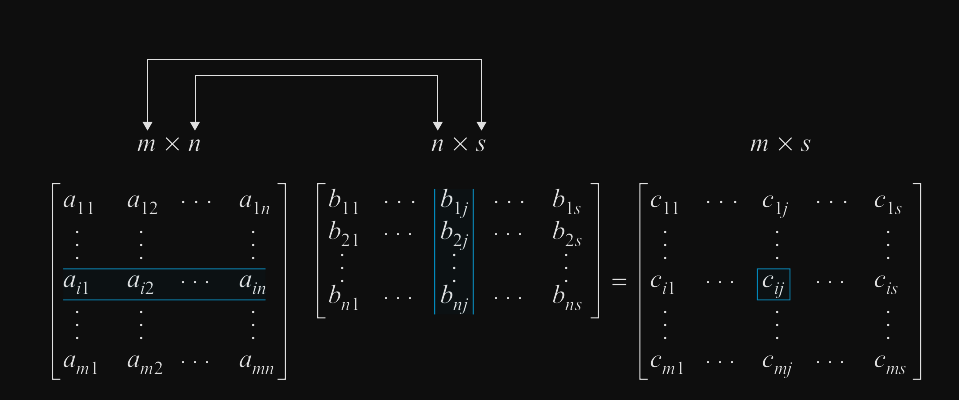
\includegraphics[scale=0.3]{./MatrixProduct.png}
\end{center}
}
%-------------- end slide -------------------------------%}}}

%-------------- start slide -------------------------------%{{{ 9
\begin{frame}[fragile]
\begin{example}
Using the above definition,
the $(\textcolor{coral}{2},\textcolor{lgtblue}{3})$-entry of the product
\[
\left[\begin{array}{rrr}
-1 & 0 & 3 \\
\textcolor{coral}{2} & \textcolor{coral}{-1} & \textcolor{coral}{1}
\end{array}\right]
\left[\begin{array}{rrr}
-1 & 1 & \textcolor{lgtblue}{2} \\
0 & -2 & \textcolor{lgtblue}{4} \\
1 & 0 & \textcolor{lgtblue}{0}
\end{array}\right]
\]
is computed by the dot product of the \textcolor{coral}{second row} of the first
matrix and the \textcolor{lgtblue}{third column} of the second matrix:
\[ \textcolor{coral}{2}\times \textcolor{lgtblue}{2} +
    (\textcolor{coral}{-1}) \times \textcolor{lgtblue}{4} +
\textcolor{coral}{1}\times \textcolor{lgtblue}{0} = 4-4+0=0.\]
\end{example}

\end{frame}
%-------------- end slide -------------------------------%}}}

\section[\textcolor{yellow}{}]{\textcolor{yellow}{Properties of Matrix Multiplication}}

%-------------- start slide -------------------------------%{{{ 10
\frame{
\frametitle{Properties of Matrix Multiplication}
\pause
\begin{emptytitle}
    Given matrices $A$ and $B$, is $AB=BA$?
\end{emptytitle}
}
%-------------- end slide -------------------------------%}}}

%-------------- start slide -------------------------------%{{{ 11
\frame{
\begin{problem}
    Let
    \[
	A= \left[\begin{array}{rr}
	    1  & 2 \\
	    -3 & 0 \\
	    1  & -4 \\
	\end{array}\right]
	\quad\text{and}\quad
	B= \left[\begin{array}{rrrr}
	    1 & -1 & 2 & 0 \\
	    3 & -2 & 1 & -3 \\
	\end{array}\right]
    \]

    \begin{itemize}
	\item Does $AB$ exist?  If so, compute it.
	\item Does $BA$ exist?  If so, compute it.
    \end{itemize}
\end{problem}
\pause
\vfill
\begin{solution}
    \pause
    \[ AB =
    \left[\begin{array}{rrrr}
	7   & -5 & 4  & -6 \\
	-3  & 3  & -6 & 0  \\
	-11 & 7  & -2 & 12
    \end{array}\right] \]
    \pause
    \alert{
    \[ BA \mbox{ does not exist!}\] }
    \myQED
\end{solution}
}
%-------------- end slide -------------------------------%}}}

%-------------- start slide -------------------------------%{{{ 12
\frame{
\begin{problem}
    Let
    \[
    G= \left[\begin{array}{r}
    1 \\ 1
    \end{array}\right]
    \quad\text{and}\quad
    H= \left[\begin{array}{rr}
    1 & 0
    \end{array}\right] \]

    \begin{itemize}
	\item Does $GH$ exist?  If so, compute it.
	\item Does $HG$ exist?  If so, compute it.
    \end{itemize}
\end{problem}
\pause
\vfill
\begin{solution}
    \pause
    \[ GH = \left[\begin{array}{rr}
    1 & 0 \\ 1 & 0
    \end{array}\right] \]
    \pause
    \[ HG = \left[\begin{array}{r} 1 \end{array}\right] \]
\end{solution}
\pause
\begin{remark}
    In this example, $GH$ and $HG$ both exist, but they are not equal.
    They aren't even the same size!
\end{remark}
}
%-------------- end slide -------------------------------%}}}

%-------------- start slide -------------------------------%{{{ 13
\frame{
\begin{problem}
    Let
    \[
	P= \left[\begin{array}{rr} 1 & 0 \\ 2 & -1 \end{array}\right] \quad\text{and}\quad
	Q= \left[\begin{array}{rr} -1 & 1 \\ 0 & 3 \end{array}\right] \]
    \begin{itemize}
	\item Does $PQ$ exist?  If so, compute it.
	\item Does $QP$ exist?  If so, compute it.
    \end{itemize}
\end{problem}
\pause
\vfill
\begin{solution}
    \pause
    \[ PQ = \left[\begin{array}{rr}
    -1 & 1 \\ -2 & -1
    \end{array}\right] \]
    \pause
    \[ QP = \left[\begin{array}{rr}
    1 & -1 \\ 6 & -3
    \end{array}\right] \]
    \myQED
\end{solution}
\pause
\vfill
\begin{remark}
    In this example, $PQ$ and $QP$ both exist and are the same size, but $PQ\neq QP$.
\end{remark}
}
%-------------- end slide -------------------------------%}}}

%-------------- start slide -------------------------------%{{{ 14
\frame{
\begin{fact}
The three preceding problems illustrate an important
property of matrix multiplication.
\vspace{1em}

\begin{quote}
In general, matrix multiplication is \alert{not}
commutative, i.e., the order of the matrices in the
product is important.
\end{quote}

\vspace{1em}
In other words, in general $$\alert{AB \neq BA}.$$
\end{fact}
\vfill

\begin{center}
    \textcolor{teal}{Multiplying from left or right, it MATTERS!}
\end{center}
}
%-------------- end slide -------------------------------%}}}

%-------------- start slide -------------------------------%{{{ 15
\frame{
\begin{problem}
    Let
    \[
    U= \left[\begin{array}{rr}
    2 & 0 \\ 0 & 2
    \end{array}\right]
    \quad\text{and}\quad
    V= \left[\begin{array}{rr}
    1 & 2 \\ 3 & 4
    \end{array}\right]
    \]
    \begin{itemize}
	\item Does $UV$ exist?  If so, compute it.
	\item Does $VU$ exist?  If so, compute it.
    \end{itemize}
\end{problem}
\pause
\vfill
\begin{solution}
    \[ UV = \left[\begin{array}{rr}
    2 & 4 \\ 6 & 8
    \end{array}\right] \]
    \pause
    \[ VU = \left[\begin{array}{rr}
    2 & 4 \\ 6 & 8
    \end{array}\right] \]
    \myQED
\end{solution}
\pause
\vfill
\begin{remark}
    In this particular example, the matrices \alert{commute,} i.e., $UV=VU$.
\end{remark}
}
%-------------- end slide -------------------------------%}}}

%-------------- start slide -------------------------------%{{{ 16
\frame{
\begin{theorem}[Properties of Matrix Multiplication]
    Let $A$, $B$, and $C$ be matrices of the appropriate sizes, and let
    $r\in\RR$ be a scalar.  Then the following properties hold.
    \pause
    \begin{enumerate}
	\item $I A = A$ and $AI=A$.
	\item $A(B+C) = AB + AC$.

	    \textcolor{blue}{(matrix multiplication distributes over matrix addition).}
	    \pause
	\item $(B+C)A = BA + CA$.

	    \textcolor{blue}{(matrix multiplication distributes over matrix addition).}
	    \pause
	\item $A\left( BC\right) =\left( AB\right) C$.
	    \textcolor{blue}{(matrix multiplication is associative).}
	    \pause
	\item $r(AB)= (rA)B = A(rB)$.
	\item $\left(AB\right)^T = B^T A^T$.
    \end{enumerate}
\end{theorem}
\pause
\vfill
\begin{remark}
    This applies to matrix-vector multiplication
    as well, since a vector is a row matrix or a column matrix.
\end{remark}
}
%-------------- end slide -------------------------------%}}}

%-------------- start slide -------------------------------%{{{ 17
\frame{
\begin{problem}
    Let $A = \leftB a_{ij} \rightB$, $B = \leftB b_{ij} \rightB$
    and $C=\leftB c_{ij} \rightB$ be three $n \times n$ matrices.
    For $1\leq i, j\leq n$
    write down a formula for the $(i,j)$-entry of each of the following matrices.
    \begin{multicols}{2}
    \begin{enumerate}
	\item AB
	\item BA
	\item A+C
	\item C(A+B)
	\item A(BC)
	\item (AB)C
    \end{enumerate}
    \end{multicols}
\end{problem}
}
%-------------- end slide -------------------------------%}}}

%-------------- start slide -------------------------------%{{{ 18
\frame{
\begin{problem}
    Let $A$ and $B$ be $m\times n$ matrices, and let $C$ be an
    $n\times p$ matrix.
    Prove that if $A$ and $B$ commute with $C$, then $A+B$
    commutes with $C$.
\end{problem}
\pause
\vfill
    \begin{proofnoend}
    We are given that $AC=CA$ and $BC=CB$.
    Consider $(A+B)C$.
    \begin{eqnarray*}
    (A+B)C & = & \pause AC + BC \\ \pause
           & = & CA + CB        \\ \pause
           & = & C(A+B)
    \end{eqnarray*}
    \pause
    Since $(A+B)C=C(A+B)$, $A+B$ commutes with $C$.
    \myQED
\end{proofnoend}
}
%-------------- end slide -------------------------------%}}}

%-------------- start slide -------------------------------%{{{ 19
\frame{
\begin{problem}
    Let $A,B$ and $C$ be $n\times n$ matrices, and suppose that
    both $A$ and $B$ commute with $C$, i.e.,
    $AC=CA$ and $BC=CB$.
    Show that $AB$ commutes with $C$.
\end{problem}
\pause
\vfill
\begin{proofnoend}
    We must show that $(AB)C=C(AB)$ given that $AC=CA$ and $BC=CB$.
    \begin{eqnarray*}
	(AB)C & = & A(BC) ~~\mbox{\small (matrix multiplication is associative)} \\
	      & = & A(CB) ~~\mbox{\small ($B$ commutes with $C$)}                \\
	      & = & (AC)B ~~\mbox{\small (matrix multiplication is associative)} \\
	      & = & (CA)B ~~\mbox{\small ($A$ commutes with $C$)}                \\
	      & = & C(AB) ~~\mbox{\small (matrix multiplication is associative)}
    \end{eqnarray*}
    Therefore, $AB$ commutes with $C$.
    \myQED
\end{proofnoend}
}
%-------------- end slide -------------------------------%}}}

%-------------- start slide -------------------------------%{{{ 20
\begin{frame}[fragile]{Partitioned matrix and block multiplication}
    \begin{block}{Observation}
        We can partition matrix into blocks so that each entry of the partitioned matrix is again a matrix.
    \end{block}
    \vfill
    \begin{example}
    \begin{center}
	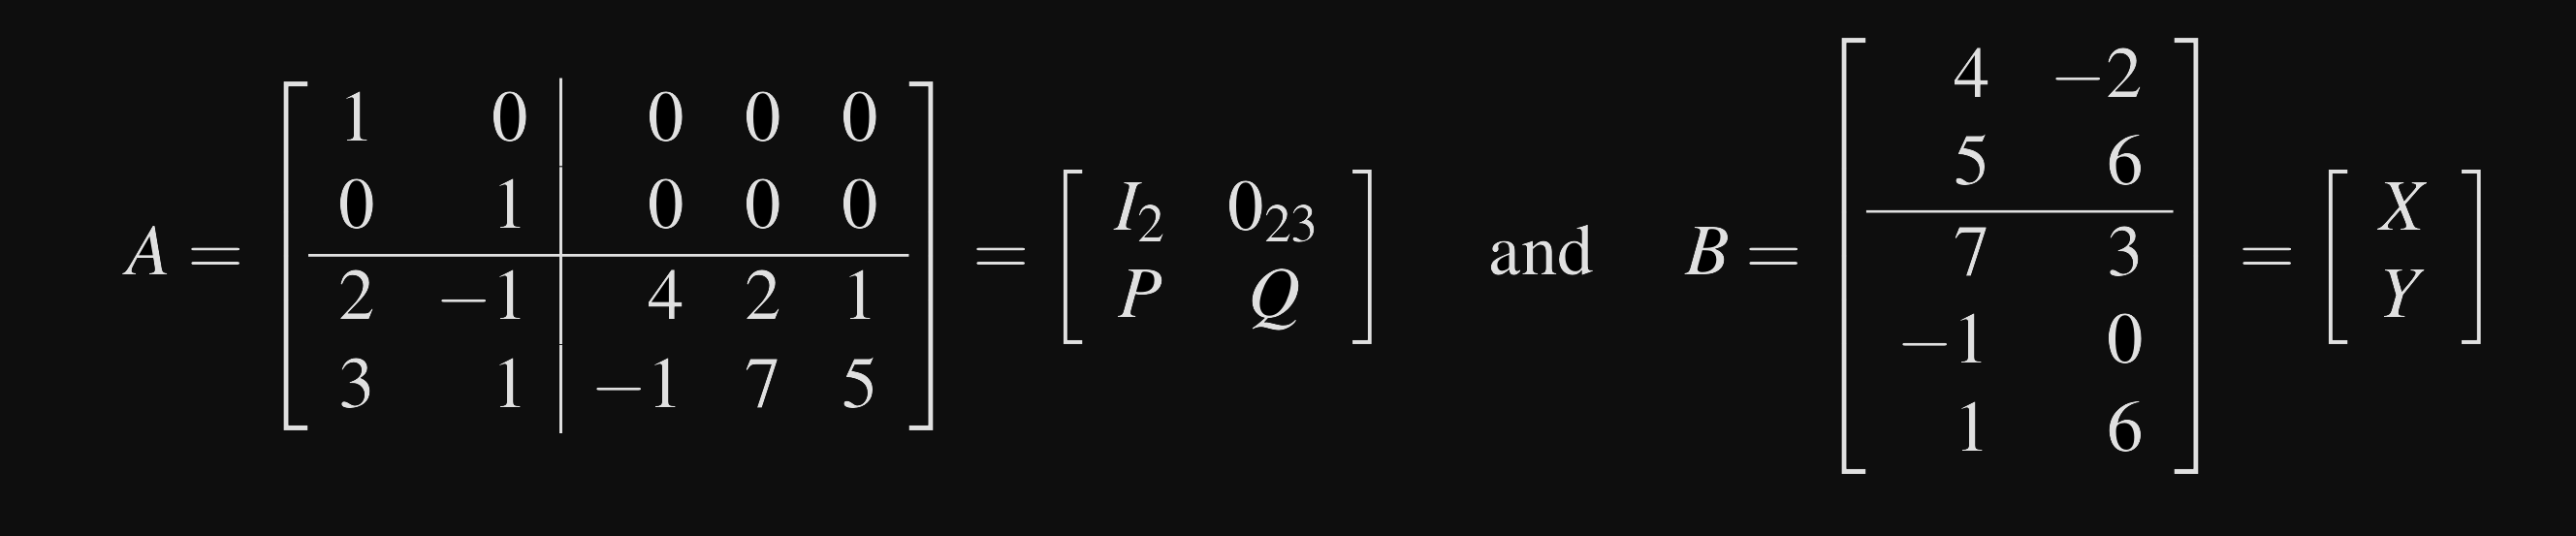
\includegraphics[scale=0.1]{./figures/Partitioned_Matrices_Examples.png}
    \end{center}
    \end{example}
\end{frame}
%-------------- end slide -------------------------------%}}}

%-------------- start slide -------------------------------%{{{ 21
\begin{frame}[fragile]

    \begin{example}
    Let $A$ and $B$ be $m\times n$ and $n\times k$ matrices, respectively.
    We can partition then into either column vectors or row vectors:
    \pause
    When viewed as partitioned matrices, $AB$ can be equivalently written in one of the following four ways:
    \vspace{1em}
    \[
	A_{mn} =
	\begin{pmatrix} \vec{a}_1,\cdots,\vec{a}_n \end{pmatrix}
	= \begin{pmatrix} \vec{\alpha}_1^T \cr \vdots\cr \vec{\alpha}_m^T \end{pmatrix}
	\quad\text{and}\quad
	B_{nk} =
	\begin{pmatrix} \vec{b}_1,\cdots,\vec{b}_k \end{pmatrix}
	= \begin{pmatrix} \vec{\beta}_1^T \cr \vdots\cr \vec{\beta}_n^T \end{pmatrix}
    \]
    \begin{enumerate}
        \item
    \[
	AB = A \begin{pmatrix} \vec{b}_1,\cdots,\vec{b}_k \end{pmatrix}  =
	    \begin{pmatrix}A \vec{b}_1,\cdots,A\vec{b}_k \end{pmatrix}
    \]
    \vfill
        \item
    \[
	AB = \begin{pmatrix} \vec{\alpha}_1^T \cr \vdots\cr \vec{\alpha}_m^T \end{pmatrix} B
	 =   \begin{pmatrix} \vec{\alpha}_1^T B\cr \vdots\cr \vec{\alpha}_m^T B\end{pmatrix}
    \]
    \end{enumerate}
    \end{example}
\end{frame}
%-------------- end slide -------------------------------%}}}

%-------------- start slide -------------------------------%{{{ 22
\begin{frame}[fragile]
    \begin{example}[continued]
    \begin{enumerate}
	\item[3]
    \[
	AB =
	\begin{pmatrix} \vec{a}_1,\cdots,\vec{a}_n \end{pmatrix}
	\begin{pmatrix} \vec{\beta}_1^T \cr \vdots\cr \vec{\beta}_n^T \end{pmatrix}
	=
	\vec{a}_1 \vec{\beta}_1^T +
	\vec{a}_2 \vec{\beta}_2^T +
	\cdots
	\vec{a}_n \vec{\beta}_n^T
    \]
    \vspace{3em}
\item[4]
    \[
	AB =
	\begin{pmatrix} \vec{\alpha}_1^T \cr \vdots\cr \vec{\alpha}_m^T \end{pmatrix}
	\begin{pmatrix} \vec{b}_1,\cdots,\vec{b}_k \end{pmatrix}
	=
	\begin{pmatrix}
	    \vec{\alpha}_1^T b_1 & \vec{\alpha}_1^T b_2 &\cdots & \vec{\alpha}_1^T b_k \\
	    \vec{\alpha}_2^T b_1 & \vec{\alpha}_2^T b_2 &\cdots & \vec{\alpha}_2^T b_k \\
	    \vdots & \vdots &\ddots & \vdots \\
	    \vec{\alpha}_m^T b_1 & \vec{\alpha}_m^T b_m &\cdots & \vec{\alpha}_m^T b_k \\
	\end{pmatrix}
    \]
    \end{enumerate}
    \end{example}
\end{frame}
%-------------- end slide -------------------------------%}}}

%-------------- start slide -------------------------------%{{{ 23
\begin{frame}[fragile]
    \begin{example}[continued]
   One can also partition $A$ and $B$ as follows:
   \[
       A = \begin{pmatrix} A_{11} & A_{12}\cr A_{21} & A_{22} \end{pmatrix}
       \quad\text{and}\quad
       B = \begin{pmatrix} B_{11} & B_{12}\cr B_{21} & B_{22} \end{pmatrix}
   \]
   in a way that dimensions match. Then
   \[
       AB = \begin{pmatrix}
	   A_{11} B_{11} + A_{12} B_{21}  & A_{11} B_{12} + A_{12} B_{22}  \\
	   A_{21} B_{11} + A_{22} B_{21}  & A_{21} B_{12} + A_{22} B_{22}
       \end{pmatrix}
   \]
\end{example}
\end{frame}
%-------------- end slide -------------------------------%}}}

%-------------- start slide -------------------------------%{{{ 24
\begin{frame}[fragile]
\begin{problem}
    Let $A$ be a square matrix.
    Compute $A^k$ where $A= \begin{pmatrix} I & X\cr O & O \end{pmatrix} $.
\end{problem}
\vfill
\begin{solution}
\begin{align*}
    A^2 = \cdots = A.
\end{align*}
Hence, $A^k=A$ for all $k\ge 2$.
\end{solution}
\end{frame}
%-------------- end slide -------------------------------%}}}

\end{document}
